\chapter{Experimental Details}

Having discussed all of the relevant theoretical aspects of the Higgs boson and its role in the Standard Model as 
well as how we can measure it in particle colliders in theory, it is now necessary to explain how this is done in 
practice. This chapter covers all experimental tools used to do so relevant to this thesis, from the Large Hadron 
Collider (LHC) that facilitates particle collisions to the ATLAS detector that records their interaction products. 
I will start with discussions about the hardware of the LHC and ATLAS and then move on to talk about object 
reconstructions within the context of our experiment.

\section{The Large Hadron Collider}

The Large Hadron Collider (LHC) is the largest proton-proton collider in the world, located at the CERN
\footnote{"Organisation européenne pour la recherche nucléaire" or in its english translation "European 
Organization for Nuclear Research"} laboratory near Geneva, Switzerland. It is a circular collider with a circumference 
of 26.7 km and can accelerate both protons and heavy ion beams to $6.8\ TeV$, leading to center of mass energies of up 
to $13.6\ TeV$ in collisions. To facilitate these collisions, the LHC accelerates two collimated beams \footnote{The 
beams are not continuous but rather consist of individual bunches that are spaced evenly} of hadrons simultaneously and 
guides them towards each other at 4 intersection points. These points correspond to the sites of the four main detectors 
located on the LHC ring: ATLAS, CMS, LHCb and ALICE. \par

%https://www.nature.com/articles/s42254-024-00758-5
\begin{figure}
\centering
    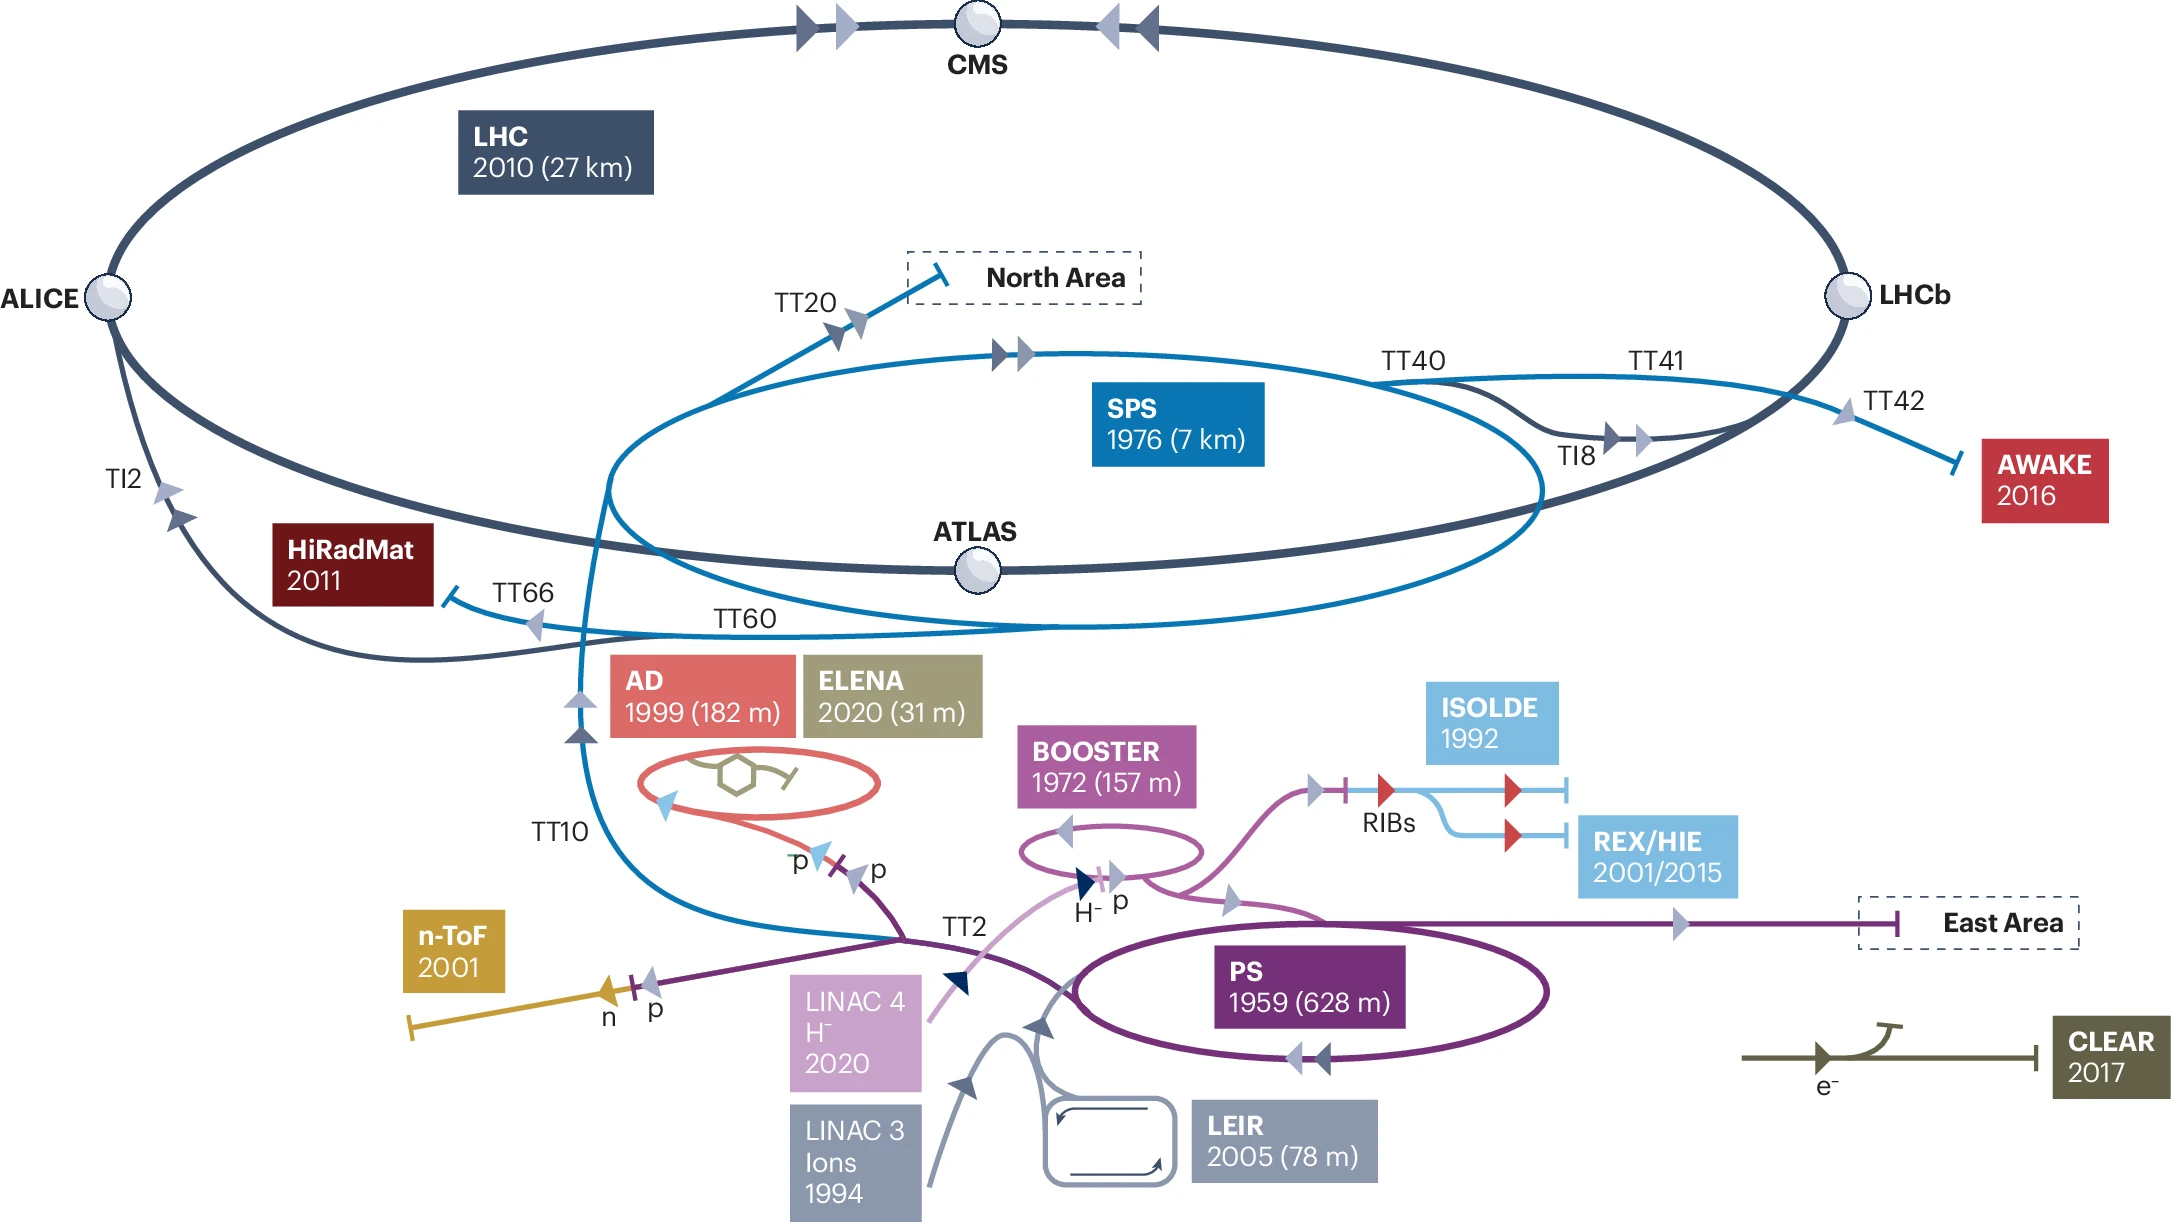
\includegraphics[width=1.0\textwidth]{images/CERN_Complex.png}
    \caption{Schematic overview of the CERN accelerator complex including main synchrotron accelerators LHC, SPS 
    and PS.}
    \label{fig:CERN_Complex}
\end{figure}

Achieving the desired collision energies requires the use of mutliple components of the CERN accelerator complex 
detailed in figure \ref{fig:CERN_Complex}, which consists of linear and smaller circular colliders that were operated 
as independent experiments in the past. The acceleration is facilitated by an intricate setup of magnets (mostly 
dipoles and quadrupoles), 
which also steer and focus the beams. For proton-proton collisions this process starts with $H^-$ ions which are 
accelerated to $160\ MeV$ by a linear accelerator called Linac4. From there the ions are injected into the circular  
Proton Synchrotron Booster (PSB), which strips both electrons from the Hydrogen ions and creates a pure proton beam with 
an energy of $2\ GeV$. Afterwards the beam is accelerated to $26\ GeV$ by the Proton Synchrotron (PS) and $450\ GeV$ by the Super Proton Synchrotron (SPS) before finally being injected into the LHC where it reaches its final collision energy. 
\par

%https://home.cern/news/news/accelerators/accelerator-report-excellent-2024-lhc-run-ended-abruptly
\begin{table}
\begin{center}
\caption{Overview of run periods of the LHC between 2008 and 2026.}
\label{table-lhc-runs}
\begin{tabular}{|c c c c|} 
 \hline
 Run Number & Years & Center of mass energy & Integrated Luminosity \\ [0.5ex] 
 \hline
 1 & 2008-2013 & $7-8\ TeV$ & $29.2\ fb^{-1}$ \\ 
 2 & 2015-2018 & $13\ TeV$ & $159.8\ fb^{-1}$ \\ 
 3 & 2022-2026 & $13.6\ TeV$ & $195.9\ fb^{-1}$ (up to and including 2024) \\ 
 \hline
\end{tabular}
\end{center}
\end{table}

The LHC has been operational since 2008, when it recorded its first proton-proton collisions at a center of mass energy 
of $7\ TeV$. Operation has been split into three distinct run periods denoted runs 1, 2 and 3 with shutdowns in 
between for maintenance and accelerator upgrades. Details on the timeline of these runs, alongside achieved energy and 
luminosity is shown in table \ref{table-lhc-runs}. Run 1 is mostly relevant for historical reasons and this thesis will 
focus on data collected during runs 2 and 3 given the much higher center of mass energy. The LHC presents the backdrop 
for the research of thousands of physicists spread across the ATLAS, CMS, ALICE and LHCb collaborations as well as 
multiple smaller teams at any given time. It is the best tool we have available to study the kinds of most fundamental 
particle interactions we are interested in.

\section{The ATLAS detector}

ATLAS (\textbf{A} \textbf{T}oroidal \textbf{L}HC \textbf{A}pparatu\textbf{S}) is the largest of the four main detectors 
around the LHC ring. It is a general purpose detector designed to record the proton-proton collision signatures 
generated in LHC collisions without focusing too heavily on any specific processes, requiring trade-offs in detector 
design. It is around 46 meters long with a diameter of 25 meters and weights 7000 tons. The detector, visualized in 
figure \ref{fig:ATLAS_detector}, consists of four main active components: an inner tracking detector, a calorimeter 
system and a muon spectrometer. Each of these components interacts differently with different types of particles, as 
summarized in figure \ref{fig:Detector_Interactions}. The inner tracking detector is responsible for precise trajectory 
measurements of charged particles and represents the most intricate part of the ATLAS detector. The calorimeter system 
is used to measure the energy of electrons and photons (electromagnetic calorimeter) as well as hadrons (hadronic 
calorimeter). Finally the muon system identifies muons penetrating the rest of the detector. In order to make accurate 
measurements of particle momentum, the ATLAS detector uses a magnet system to curve the trajectories of charged 
particles. All of these elements will be discussed in more detail in this section.

%https://cerncourier.com/a/atlas-undergoes-some-delicate-gymnastics/
\begin{figure}[h!]
\centering
    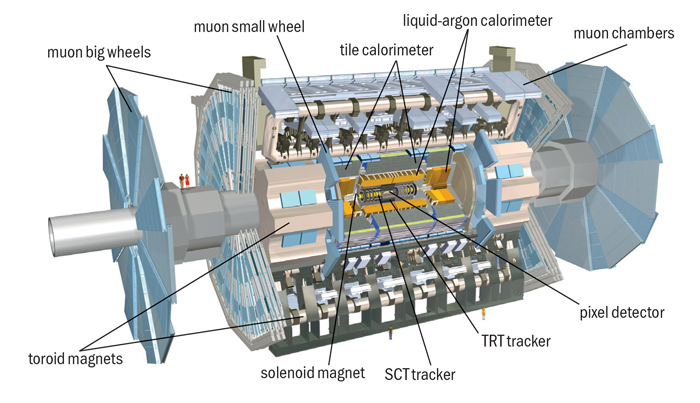
\includegraphics[width=0.8\textwidth]{images/ATLAS_Detector.jpg}
    \caption{Diagram showing all components of the ATLAS detector.}
    \label{fig:ATLAS_Detector}
\end{figure}

%https://www.nbi.dk/~petersen/Teaching/Stat2011/Project1/project1.html
\begin{figure}
\centering
    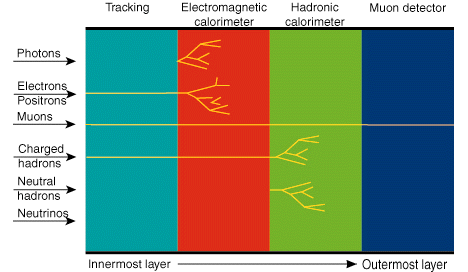
\includegraphics[width=0.8\textwidth]{images/Detector_Interactions.png}
    \caption{Sketch showing how different particles interact with detector components.}
    \label{fig:Detector_Interactions}
\end{figure}

\subsection{ATLAS coordinate system}
Before diving into the detail of the various detector components, it is important to establish the coordinate system 
used in the ATLAS experiment as well as survey physical quantities of interest related to the measurement and 
reconstruction of particle trajectories. By convention, the coordinate system is centered at the collision point, with 
the beam line representing the z-axis, the x-axis pointing towards the center of the ring and the y-axis pointing 
towards the sky, as seen in figure \ref{fig:ATLAS_Coordinate_System}. The three important coordinates related to 
particle trajectories in this spherical coordinate system are the transverse momentum $p_T$, the azimuthal angle $\phi$ 
and the pseudorapidity $\eta$. The first of these is just the momentum vector of a particle projected onto the transverse 
($xy$) plane, which also defines the azimuthal angle measured starting from the positive x-axis. The final coordinate 
$\eta$ is a measure of the longitudinal component\footnote{This is frequently referred to as the "forward component"} 
of a particle trajectory and is related to the polar angle $\theta$ by $\eta = -ln(tan(\theta/2))$. By construction, 
$\eta = 0$ if the trajectory is entirely transverse and $\eta \rightarrow \infty$ as it approaches the beamline.

%https://tikz.net/axis3d_cms/
\begin{figure}
\centering
    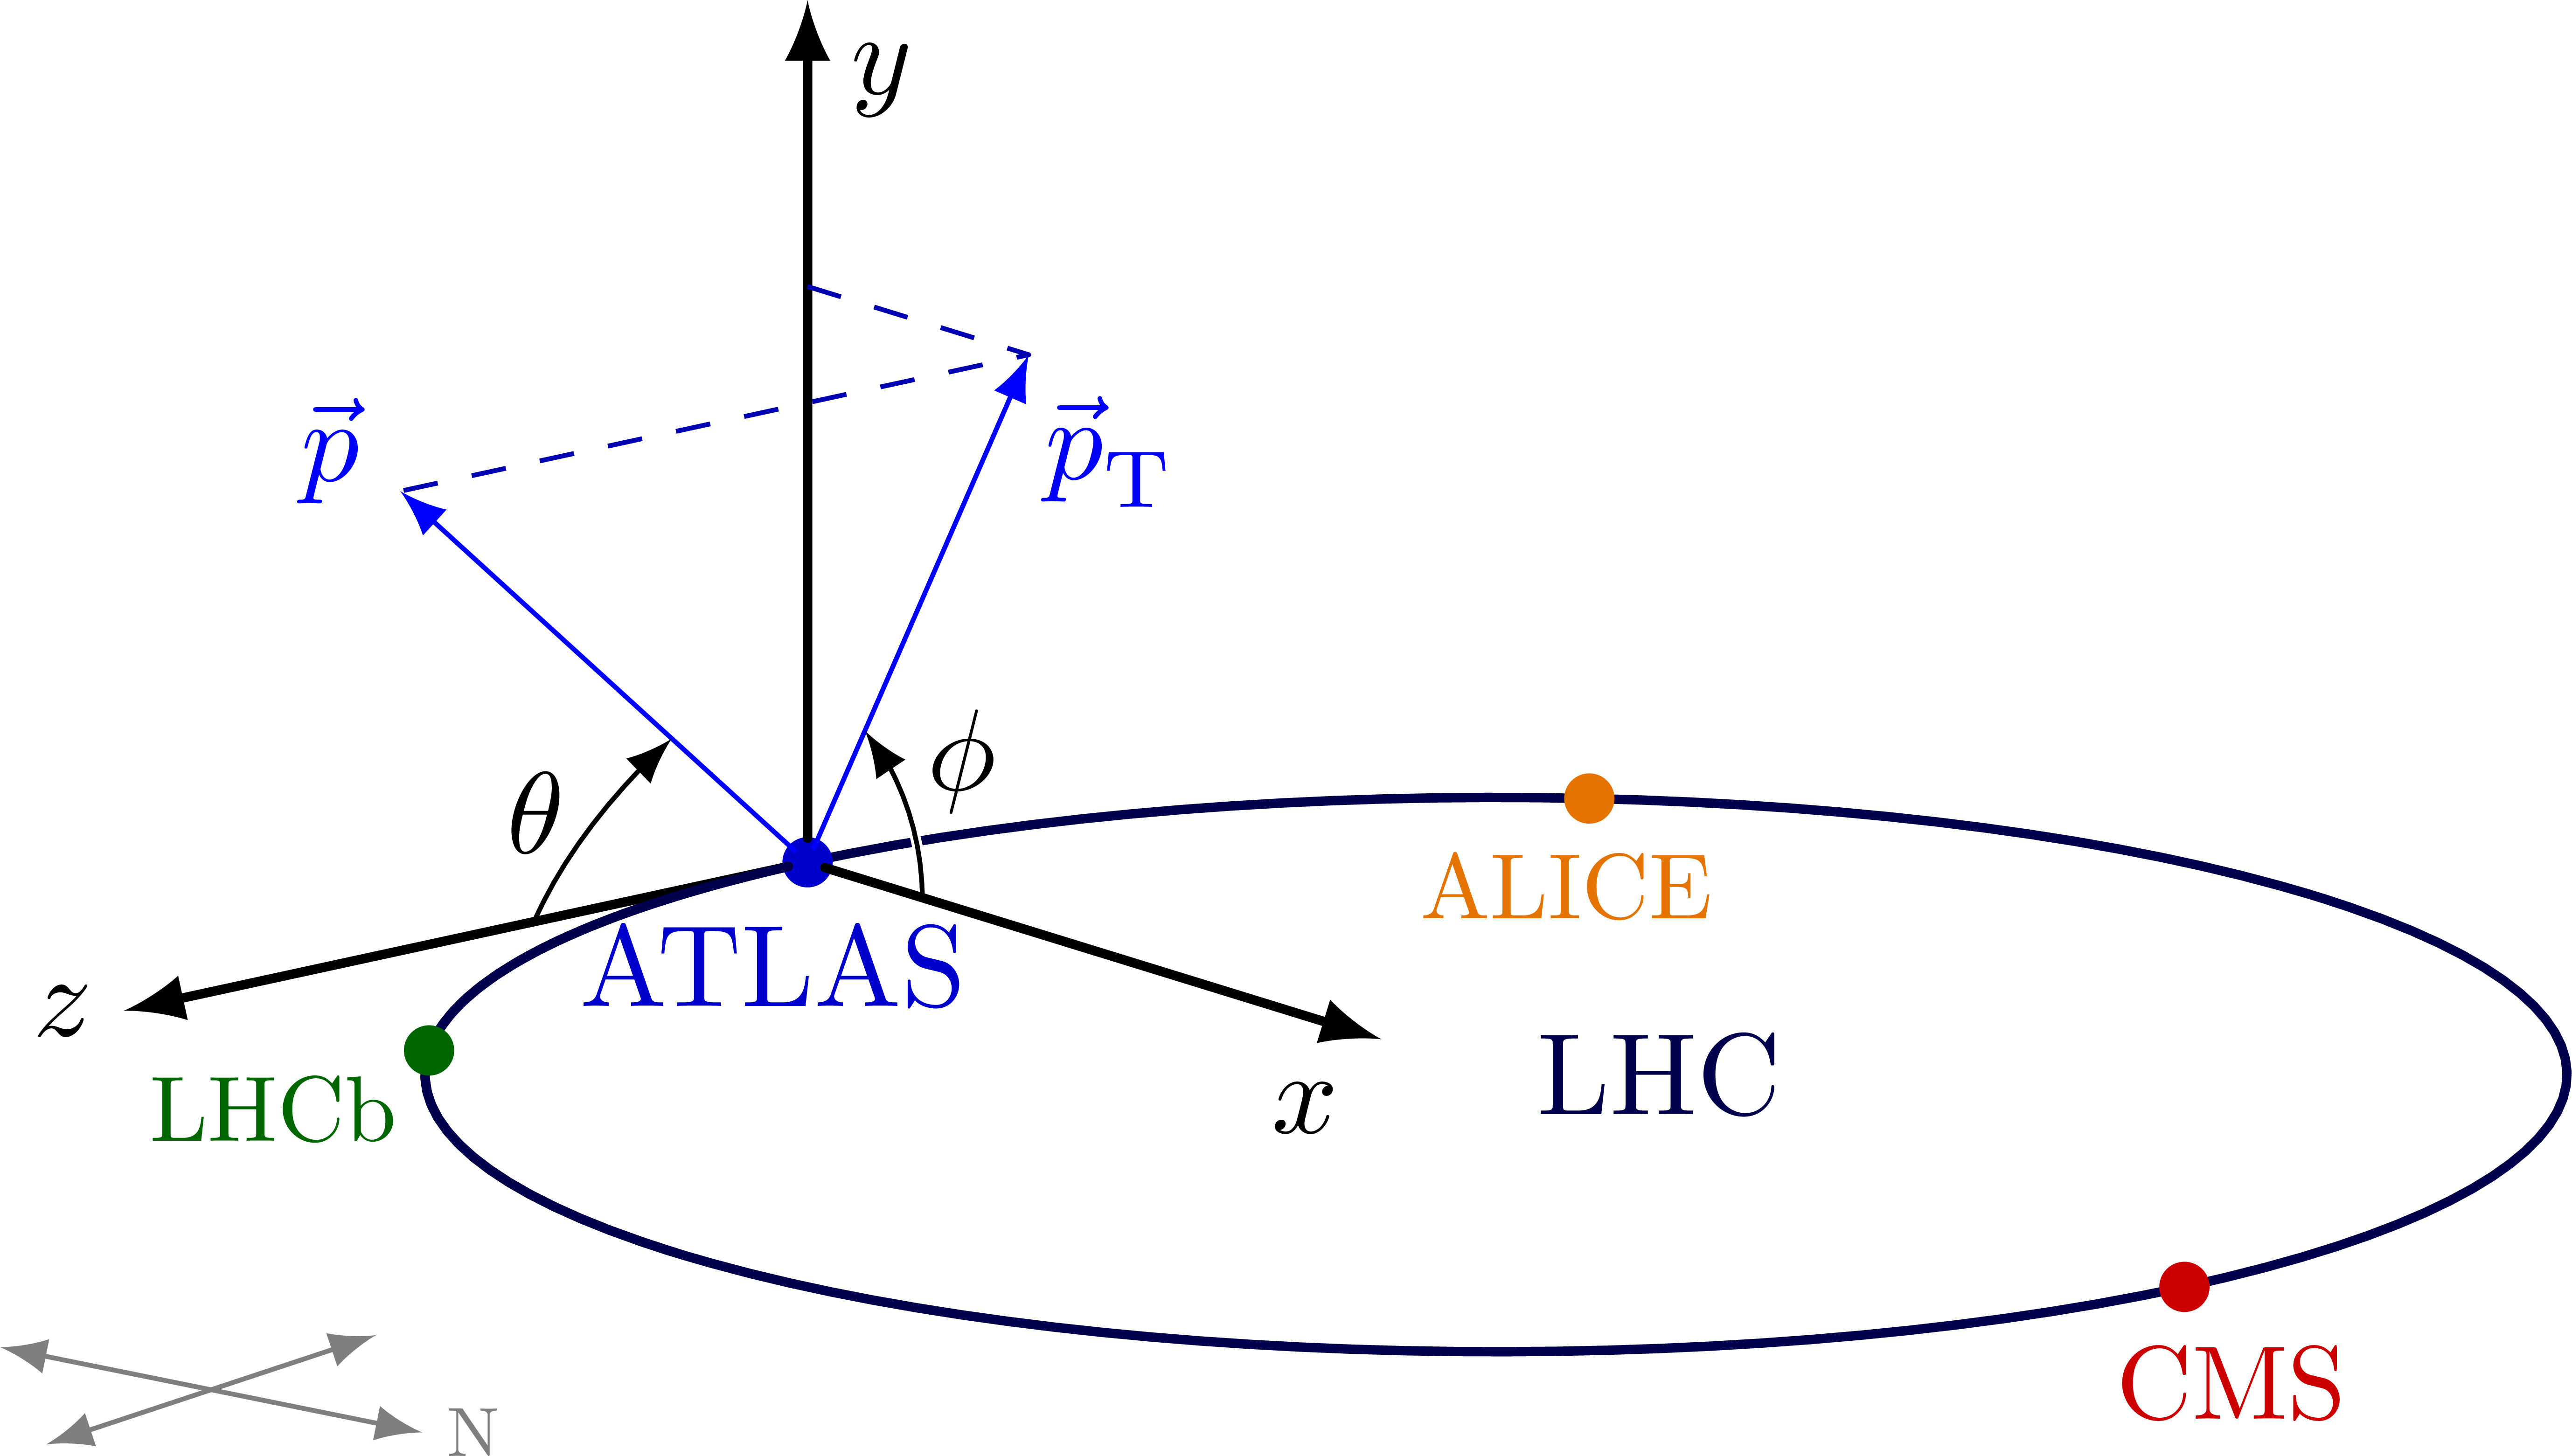
\includegraphics[width=0.6\textwidth]{images/ATLAS_Coordinate_System.png}
    \caption{Diagram showing the orientation of the coordinate system used in ATLAS as well as relevant kinematic 
    variables.}
    \label{fig:ATLAS_Coordinate_System}
\end{figure}

\subsection{Inner tracking detector}
The core of the ATLAS detector is the inner tracking detector, which is primarily responsible for precisely measuring 
the trajectories of charged particles by recording currents from electrons freed via the ionization of detector 
material. It is a combination of three different sub-systems: a pixel detector on the inside surrounded by a 
semiconductor tracker (SCT) and finally a transition radiation tracker (TRT) on the outside. The pixel detector and 
SCT are built from silicon wafers while the TRT is made up of drift tubes filled with a Xenon-based gas mixture, with 
each subsequent part of the detector providing increasingly less granular position measurements. Geometrically the 
inner detector consists of barrel and endcap components where the barrel is a cylinder covering the entire transverse 
plane within a range of $|\eta| < 2.5$ and the endcaps are disks placed on either side of the barrel to detect 
forward particles. \par

%https://atlas.cern/Discover/Detector/Inner-Detector
\begin{figure}
\centering
    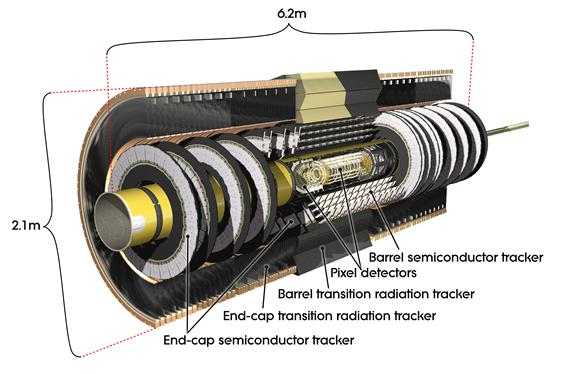
\includegraphics[width=0.6\textwidth]{images/ATLAS_Inner_Detector.jpg}
    \caption{Schematic of the ATLAS inner detector and its components.}
    \label{fig:ATLAS_Inner_Detector}
\end{figure}

The pixel detector \cite{pernegger-pixel-detector} is silicon-based and made up of a total of 92 million individual 
elements (pixels) arranged in 4 layers for the barrel component (1736 modules total) as well as 3 disk layers for each 
endcap (288 modules total). The innermost layer, called the insertable B-layer, was inserted prior to run 2 of the LHC 
and is located a distance of 3.3cm from the beam pipe. It has the smallest individual pixel elements at 
$50\times250\ \mu m^2$, allowing for increased position resolution closest to the beam. All remaining layers have 
pixels of size $50\times400\ \mu m^2$, resulting in an overall spatial resolution of $\sim 8 \mu m$ in $r\phi$ and 
$\sim 75 \mu m$ in $z$. \par

%SCT

%TRT

\subsection{Calorimeter system}

\subsection{Muon system}

\subsection{Magnet system}

\section{Object reconstruction}

\subsection{Particle tracking}

\subsection{Jet reconstruction}

\subsection{Particle identification}